\documentclass[a4paper,12pt]{article}
\usepackage{amsmath}
\usepackage{pdfpages}
\usepackage[utf8]{inputenc}
\usepackage{hyperref}
\usepackage{listings}
\usepackage{xcolor}
\usepackage{fancyhdr}
 
\definecolor{codegreen}{rgb}{0,0.6,0}
\definecolor{codegray}{rgb}{0.5,0.5,0.5}
\definecolor{backcolour}{rgb}{0.95,0.95,0.92}

\lstdefinestyle{mystyle}{
    backgroundcolor=\color{backcolour},   
    commentstyle=\color{codegreen},
    keywordstyle=\color{blue},
    numberstyle=\tiny\color{codegray},
    basicstyle=\ttfamily\footnotesize,
    breakatwhitespace=false,         
    breaklines=true,                 
    captionpos=b,                    
    keepspaces=true,                 
    numbers=left,                    
    numbersep=5pt,                  
    showspaces=false,                
    showstringspaces=false,
    showtabs=false,                  
    tabsize=2
}

\lstset{style=mystyle}

\pagestyle{fancy}
\fancyhf{}
\lhead{Contol theory Homework \#3 report}
\rhead{Anton Brisilin, BS18-02 Student, \\ 
a.brisilin@innopolis.university}
\fancyfoot[R]{\today}
\fancyfoot[C]{\thepage}
\renewcommand{\footrulewidth}{1pt}
\renewcommand{\headrulewidth}{1pt}

\begin{document}
\section{Task 1.}
My name is \textit{Anton Brisilin}, and my email is 
\textit{a.brisilin@innopolis.university}. 
My generated variant is \textbf{F}.
\section{Task 2.}
    \subsection*{Part A.}
        Design PD-controller that tracks time varying reference states, i.e.
        \\ $[x^*(t), \dot{x}^*(t)]$ as closely as possible. Test your controller on different
        trajectories, at least two. System: $x + \mu x + kx = u$, see variants below.\\
        For variant F, $\mu = 63, k = 15$
        Our open-loop system equation is 
        \begin{equation*}
            \ddot{x}+63\dot{x}+15x=u,
        \end{equation*}
        where $x=x(t)$, $u=u(t)$\\
        Our controller is required to be PD-controller. Hence, we have following formula
        for our input $u(t)$:
        \begin{equation*}
            u(t) = K_p e(t) + K_d\dot{e}(t)
        \end{equation*}
        As I will use \texttt{odeint()} function from \texttt{scipy.integrate} module,
        I will need a formula for a derivative vector of $\vec{x} = [x(t),\dot{x}(t)]^T$: 
        $\dot{\vec{x}} = [\dot{x}(t),\ddot{x}(t)]^T$. Hence I should convert my system to 
        state-space form.
        \begin{equation*}
            \begin{bmatrix}
                \dot{x}(t)\\
                \ddot{x}(t)
            \end{bmatrix}
            = 
            \begin{bmatrix}
                0 & 1 \\
                -15 & -63
            \end{bmatrix}
            \begin{bmatrix}
                x(t)\\
                \dot{x}(t)
            \end{bmatrix}
            +
            \begin{bmatrix}
                0 \\
                1
            \end{bmatrix}
            u
        \end{equation*}
        Adding our controller, we get 
        \begin{equation*}
            \begin{bmatrix}
                \dot{x}(t)\\
                \ddot{x}(t)
            \end{bmatrix}
            = 
            \begin{bmatrix}
                0 & 1 \\
                -15 & -63
            \end{bmatrix}
            \begin{bmatrix}
                x(t)\\
                \dot{x}(t)
            \end{bmatrix}
            +
            \begin{bmatrix}
                0 \\
                1
            \end{bmatrix}
            \begin{bmatrix}
                K_p & K_d
            \end{bmatrix}
            \left(
            \begin{bmatrix}
                x^*(t)\\
                \dot{x^*}(t)
            \end{bmatrix}
            -
            \begin{bmatrix}
                x(t)\\
                \dot{x}(t)
            \end{bmatrix}
            \right)
        \end{equation*}
        Now my goal is implement such a system in Python, you can find it in 
        \texttt{Task2/pd.py}. First of all, I declared $\mu$, k, right time 
        boudary and step for numerical solution as constants
        \lstinputlisting[language = Python, firstline=5, lastline=9]{../Task2/pd.py}
        Then I declared reference functions:
        \lstinputlisting[language = Python, firstline=18, lastline=22]{../Task2/pd.py}
        Then, I created a function that will compute our derivative vector (I think 
        this is most interesting part):
        \lstinputlisting[language = Python, firstline=30, lastline=34]{../Task2/pd.py}
        Using these functions, I can simulate work of the system, and try to tune the 
        coeffitients:
        \lstinputlisting[language = Python, firstline=36, lastline=53]{../Task2/pd.py}
        \subsubsection*{Testing on different trajectories}
            As a first reference trajectory I have chosen $x^*(t)=sin(t) + t$, 
            $\dot{x}^*(t) = cos(t)+1$, with zero initial conditions. Here are the plots 
            of solution, obtained with $K_p = 5$, $K_d = 5$.
            \begin{center}
                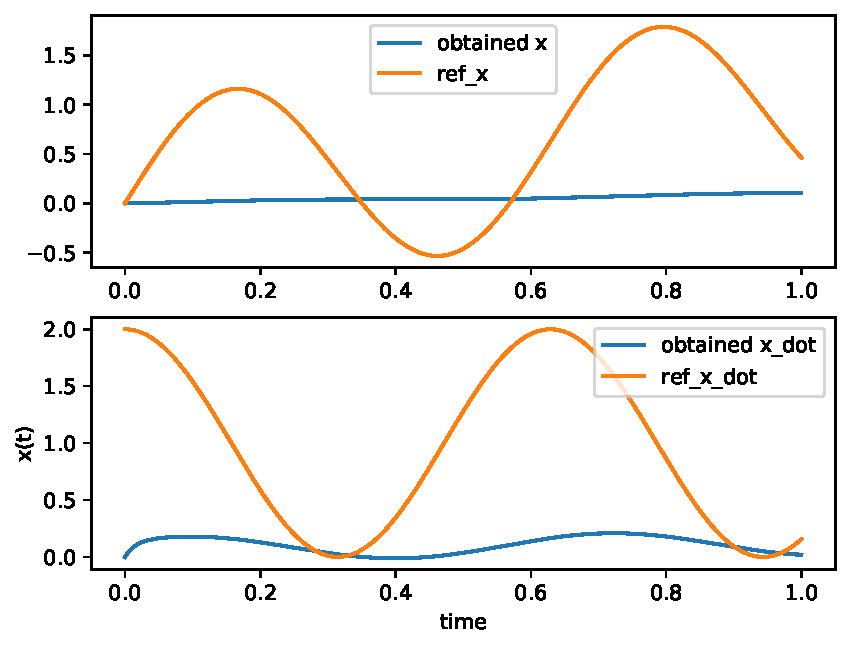
\includegraphics[width = 0.8\linewidth]{2a_tr1.pdf}
            \end{center}
            As a second reference trajectory I have chosen $x^*(t)=sin(10t)$, 
            $\dot{x}^*(t) = cos(10t)$, with zero initial conditions. Here are the plots 
            of solution, obtained with $K_p = 5$, $K_d = 5$.
            \begin{center}
                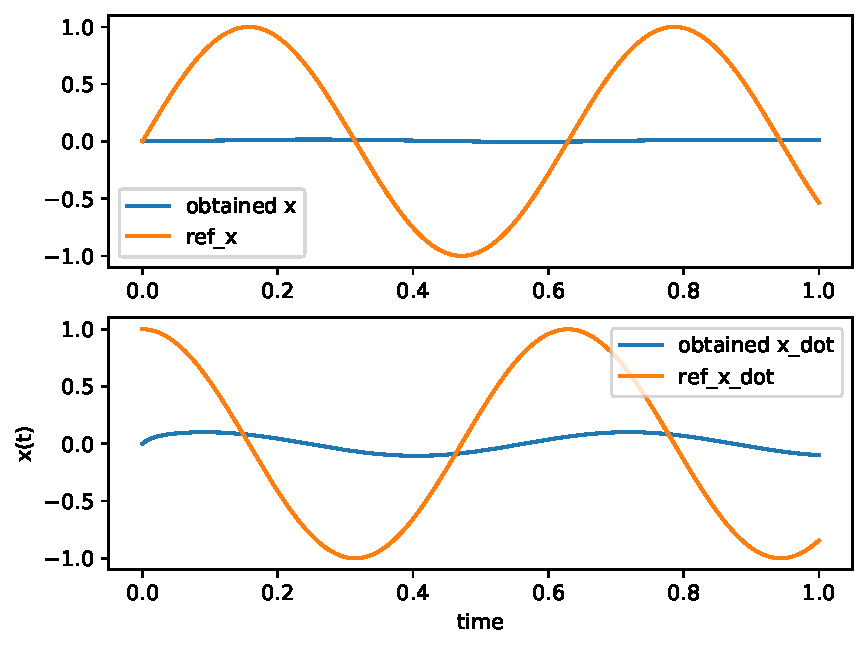
\includegraphics[width = 0.8\linewidth]{2a_tr2.pdf}
            \end{center}
            Third reference trajectory is just a step function $x^*(t)=1$, $\dot{x}^*(t) = 0$,
            with zero initial conditions. Here are the plots of solution, obtained with 
            $K_p = 5$, $K_d = 5$.
            \begin{center}
                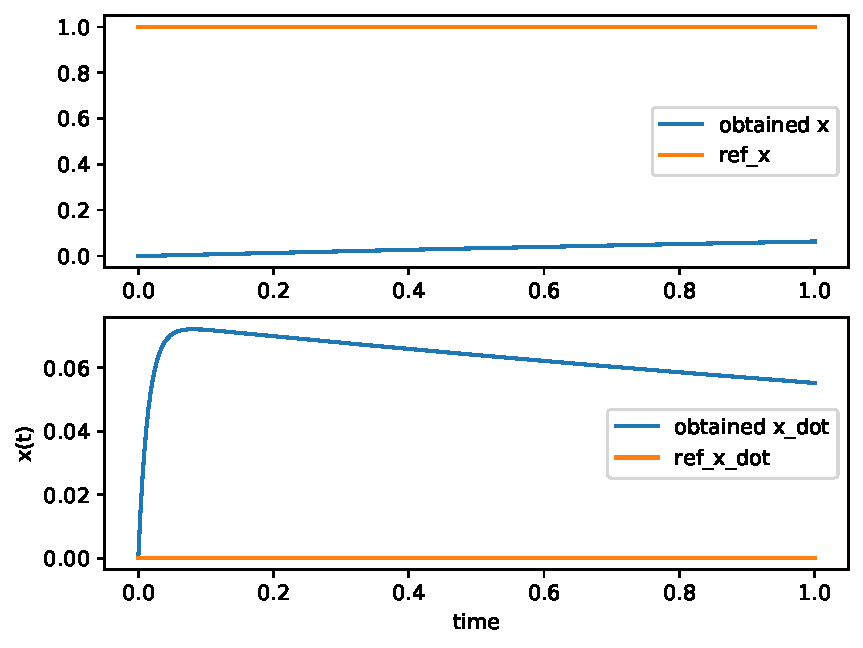
\includegraphics[width = 0.8\linewidth]{2a_tr3.pdf}
            \end{center}
            As one can see, my controller poorly follows desired trajectory and need
            to be tuned for each trajectory individually. 
    \subsection*{Part B. Controller tuning}
        We begin with $K_p = 5$, $K_d = 5$. As you can see on the above plot, 
        it gives us a large steady - state error, so $K_p$ should be increased.\\ 
        I increased it, 
        until I got steady-state error $e \approx 10^{-2}$. The values are 
        $K_p = 2000$, $K_d = 5$
        \begin{center}
            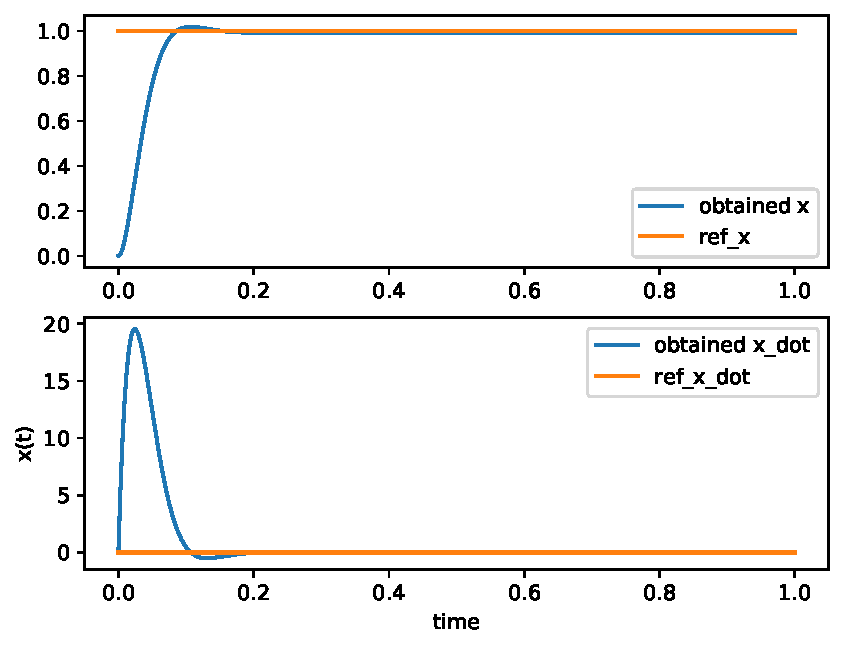
\includegraphics[width = 0.72\linewidth]{2b_1.pdf}
        \end{center}
        Now we have almost no steady-state error, but there is an overshoot now.
        Therefore, $K_d$ should be increased.\\
        I increased it, until I got rid of overshoot. The values are 
        $K_p = 2000$, $K_d = 13$
        \begin{center}
            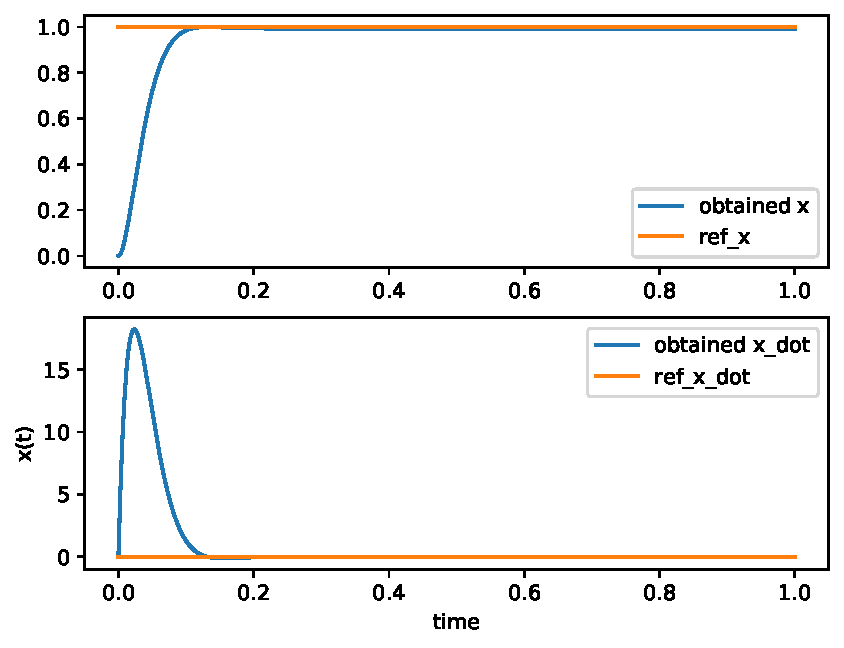
\includegraphics[width = 0.77\linewidth]{2b_2.pdf}
        \end{center}
        Now there is no overshoot, and steady-state error $e \approx 10^{-2}$, 
        as it can bee seen from the plot. The gains are $K_p = 2000$, $K_d = 13$.
    \subsection*{Part C. Proving stability}
        For the controlled system 
        \begin{equation*}
            \begin{cases}
                \dot{x}=Ax+Bu\\
                u = -Kx
            \end{cases}
        \end{equation*}
        to be stable, all real parts of eigenvalues of matrix $[A-BK]$ should be
        negative. In our case, we have
        \begin{equation*}
            \begin{cases}
                \dot{x}=
                \begin{bmatrix}
                    0 & 1 \\
                    -15 & -63
                \end{bmatrix}
                x+
                \begin{bmatrix}
                    0 \\
                    1
                \end{bmatrix}
                u
                \\
                \\
                u = -
                \begin{bmatrix}
                    K_p & K_d
                \end{bmatrix}
                e
            \end{cases}
        \end{equation*}
        \begin{eqnarray*}
            A-BK = 
            \begin{bmatrix}
                0 & 1 \\
                -15 & -63
            \end{bmatrix}
            -
            \begin{bmatrix}
                0 \\
                1
            \end{bmatrix}
            \begin{bmatrix}
                2000 & 13
            \end{bmatrix}\\
            \\
            A-BK = 
            \begin{bmatrix}
                0 & 1 \\
                -15 & -63
            \end{bmatrix}
            -
            \begin{bmatrix}
                0 & 0\\
                2000 & 13
            \end{bmatrix}\\
            \\
            A-BK = 
            \begin{bmatrix}
                0 & 1 \\
                -2015 & -76
            \end{bmatrix}
        \end{eqnarray*}
        Using Matlab's \texttt{eig()} function, I obtained the eigenvalues, that 
        are
        \begin{equation*}
            eigenvalues = 
            \begin{bmatrix}
                -38 + 23.8956i\\
                -38 - 23.8956i
            \end{bmatrix}
        \end{equation*}
        As it can be seen, they have negative real parts, so the controlled system
        is stable.
    \subsection*{Part D.}
    Think of how you would implement PD control for a linear system:
    \begin{equation*}
        \begin{bmatrix}
            \dot{x_1}\\
            \dot{x_2}
        \end{bmatrix}
        = 
        \begin{bmatrix}
            10 & 3 \\
            5 & -5
        \end{bmatrix}
        \begin{bmatrix}
            x_1\\
            x_2
        \end{bmatrix}
    \end{equation*}
    This system is autonomous MIMO system. I need to add controller to it to 
    make it stable. First of all, let's check its stability by looking to its 
    eigenvalues, obtained with Python's \texttt{numply.linalg.eig()}.
    \begin{equation*}
        eigenvalues = 
        \begin{bmatrix}
            10.94\\
            -5.94
        \end{bmatrix}
    \end{equation*}
    As can be seen, it is unstable, because it has eigenvalue with positive
    real part. Thus, we need to add controller to the system. We do not want our 
    system to keep any trajectory, we just want to stabilize it. Therefore, we 
    want $\dot{x}$ go to zero in equation
    \begin{equation*}
        \dot{x} = Ax + B(K_px + K_d\dot{x}),
    \end{equation*}
    where $K_p$ and $K_d$ are proportional and derivative gains respectively, and
    $x$ is state vector.\\
    If we want to implement that system, we should express $\dot{x}$ in terms of
    $x$
    \begin{eqnarray*}
        \dot{x} = Ax + B(K_px + K_d\dot{x})\\
        \dot{x} = (A + BK_p)x + BK_d\dot{x}\\
        (I-BK_d)\dot{x}= (A + BK_p)x\\
        \dot{x}= (I-BK_d)^{-1}(A + BK_p)x\\
    \end{eqnarray*}
    But if we pick differential gain $K_d = B^{-1}$, our equation will look like
    \begin{equation*}
        0 = (A + BK_p)x
    \end{equation*}
    That means that implemented PD control is applicable only to $x \in N(A+BK_p)$,
    i.e. such vectors $x$ that are in nullspace of $A+BK_p$. Hence, implemented 
    controller is not suitable for us. 
    \subsection*{Part E.} 
\section{Used software.}
\begin{itemize}
    \item Python 3.8.1
    \item Matlab R2018b 9.5.0
\end{itemize}
All software was run under Manjaro Linux with 5.4.18-rt kernel
\end{document}